% Önálló forrás; fordítás: xelatex soma-feladatlap.tex
\documentclass[a4paper,10pt]{article}
\usepackage[margin=14mm]{geometry}
\usepackage{fontspec}
\setmainfont{Latin Modern Roman}
\usepackage{babel}
\babelprovide[main,import]{hungarian}
\usepackage{tikz,multicol}
\setlength{\parindent}{0pt}
\setlength{\columnsep}{8mm}
\definecolor{soma1}{HTML}{32934b}
\definecolor{soma2}{HTML}{337ac5}
\definecolor{soma3}{HTML}{f3cc32}
\definecolor{soma4}{HTML}{242424}
\definecolor{soma5}{HTML}{d63832}
\definecolor{soma6}{HTML}{ffffff}
\definecolor{soma7}{HTML}{8843b5}
\begin{document}
{\large\bfseries Soma — feladatlap}\hfill Név: \makebox[40mm]{\dotfill}\par\smallskip
{\scriptsize Elemek: 1 V (zöld), 2 L (kék), 3 T (sárga), 4 Z (fekete), 5 Ágas (piros), 6 Csavar A (fehér), 7 Csavar B (lila).\par
A rétegek alulról felfelé következnek; a rétegrajzon hátul van fent, elöl lent. A pont üres hely.}\par\medskip
\begin{multicols}{2}
\begin{minipage}{\linewidth}
\textbf{1.} Építs testet a három színezetlen nézet alapján a megadott hét elemből! A sötét mező azt jelenti, hogy azon a nézési vonalon van legalább egy kocka; a világos mezőn nincs. Mindhárom nézetnek egyszerre kell megfelelned. Bármely ilyen összeállítás helyes. A kockák lapokon keresztül alkossanak egyetlen összefüggő építményt.\par
{\scriptsize Elemek: 1, 2, 3, 4, 5, 6, 7.}\par\smallskip
\begin{center}
\begin{minipage}[t]{.31\linewidth}\centering{\scriptsize Balról}\par\smallskip
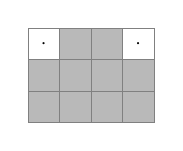
\begin{tikzpicture}[x=0.4cm,y=0.4cm]
\filldraw[fill=white,draw=gray,line width=.25pt] (0,0) rectangle ++(1,-1);
\node[font=\scriptsize] at (0.5,-0.5) {$\cdot$};
\filldraw[fill=gray!55,draw=gray,line width=.25pt] (1,0) rectangle ++(1,-1);
\filldraw[fill=gray!55,draw=gray,line width=.25pt] (2,0) rectangle ++(1,-1);
\filldraw[fill=white,draw=gray,line width=.25pt] (3,0) rectangle ++(1,-1);
\node[font=\scriptsize] at (3.5,-0.5) {$\cdot$};
\filldraw[fill=gray!55,draw=gray,line width=.25pt] (0,-1) rectangle ++(1,-1);
\filldraw[fill=gray!55,draw=gray,line width=.25pt] (1,-1) rectangle ++(1,-1);
\filldraw[fill=gray!55,draw=gray,line width=.25pt] (2,-1) rectangle ++(1,-1);
\filldraw[fill=gray!55,draw=gray,line width=.25pt] (3,-1) rectangle ++(1,-1);
\filldraw[fill=gray!55,draw=gray,line width=.25pt] (0,-2) rectangle ++(1,-1);
\filldraw[fill=gray!55,draw=gray,line width=.25pt] (1,-2) rectangle ++(1,-1);
\filldraw[fill=gray!55,draw=gray,line width=.25pt] (2,-2) rectangle ++(1,-1);
\filldraw[fill=gray!55,draw=gray,line width=.25pt] (3,-2) rectangle ++(1,-1);
\end{tikzpicture}\end{minipage}\hfill
\begin{minipage}[t]{.31\linewidth}\centering{\scriptsize Elölről}\par\smallskip
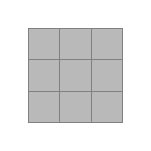
\begin{tikzpicture}[x=0.4cm,y=0.4cm]
\filldraw[fill=gray!55,draw=gray,line width=.25pt] (0,0) rectangle ++(1,-1);
\filldraw[fill=gray!55,draw=gray,line width=.25pt] (1,0) rectangle ++(1,-1);
\filldraw[fill=gray!55,draw=gray,line width=.25pt] (2,0) rectangle ++(1,-1);
\filldraw[fill=gray!55,draw=gray,line width=.25pt] (0,-1) rectangle ++(1,-1);
\filldraw[fill=gray!55,draw=gray,line width=.25pt] (1,-1) rectangle ++(1,-1);
\filldraw[fill=gray!55,draw=gray,line width=.25pt] (2,-1) rectangle ++(1,-1);
\filldraw[fill=gray!55,draw=gray,line width=.25pt] (0,-2) rectangle ++(1,-1);
\filldraw[fill=gray!55,draw=gray,line width=.25pt] (1,-2) rectangle ++(1,-1);
\filldraw[fill=gray!55,draw=gray,line width=.25pt] (2,-2) rectangle ++(1,-1);
\end{tikzpicture}\end{minipage}\hfill
\begin{minipage}[t]{.31\linewidth}\centering{\scriptsize Felülről}\par\smallskip
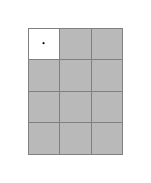
\begin{tikzpicture}[x=0.4cm,y=0.4cm]
\filldraw[fill=white,draw=gray,line width=.25pt] (0,0) rectangle ++(1,-1);
\node[font=\scriptsize] at (0.5,-0.5) {$\cdot$};
\filldraw[fill=gray!55,draw=gray,line width=.25pt] (1,0) rectangle ++(1,-1);
\filldraw[fill=gray!55,draw=gray,line width=.25pt] (2,0) rectangle ++(1,-1);
\filldraw[fill=gray!55,draw=gray,line width=.25pt] (0,-1) rectangle ++(1,-1);
\filldraw[fill=gray!55,draw=gray,line width=.25pt] (1,-1) rectangle ++(1,-1);
\filldraw[fill=gray!55,draw=gray,line width=.25pt] (2,-1) rectangle ++(1,-1);
\filldraw[fill=gray!55,draw=gray,line width=.25pt] (0,-2) rectangle ++(1,-1);
\filldraw[fill=gray!55,draw=gray,line width=.25pt] (1,-2) rectangle ++(1,-1);
\filldraw[fill=gray!55,draw=gray,line width=.25pt] (2,-2) rectangle ++(1,-1);
\filldraw[fill=gray!55,draw=gray,line width=.25pt] (0,-3) rectangle ++(1,-1);
\filldraw[fill=gray!55,draw=gray,line width=.25pt] (1,-3) rectangle ++(1,-1);
\filldraw[fill=gray!55,draw=gray,line width=.25pt] (2,-3) rectangle ++(1,-1);
\end{tikzpicture}\end{minipage}
\end{center}
\end{minipage}\par\medskip

\begin{minipage}{\linewidth}
\textbf{2.} Építs testet a három színezett nézet alapján a megadott hét elemből! A szín mindig a hozzád legközelebbi kockáé. Minden elemet pontosan egyszer használj; több, az összes nézetnek megfelelő összeállítás is helyes lehet. A kockák lapokon keresztül alkossanak egyetlen összefüggő építményt.\par
{\scriptsize Elemek: 1, 2, 3, 4, 5, 6, 7.}\par\smallskip
\begin{center}
\begin{minipage}[t]{.31\linewidth}\centering{\scriptsize Balról}\par\smallskip
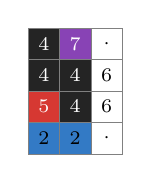
\begin{tikzpicture}[x=0.4cm,y=0.4cm]
\filldraw[fill=soma4,draw=gray,line width=.25pt] (0,0) rectangle ++(1,-1);
\node[font=\scriptsize,text=white] at (0.5,-0.5) {4};
\filldraw[fill=soma7,draw=gray,line width=.25pt] (1,0) rectangle ++(1,-1);
\node[font=\scriptsize,text=white] at (1.5,-0.5) {7};
\filldraw[fill=white,draw=gray,line width=.25pt] (2,0) rectangle ++(1,-1);
\node[font=\scriptsize] at (2.5,-0.5) {$\cdot$};
\filldraw[fill=soma4,draw=gray,line width=.25pt] (0,-1) rectangle ++(1,-1);
\node[font=\scriptsize,text=white] at (0.5,-1.5) {4};
\filldraw[fill=soma4,draw=gray,line width=.25pt] (1,-1) rectangle ++(1,-1);
\node[font=\scriptsize,text=white] at (1.5,-1.5) {4};
\filldraw[fill=soma6,draw=gray,line width=.25pt] (2,-1) rectangle ++(1,-1);
\node[font=\scriptsize,text=black] at (2.5,-1.5) {6};
\filldraw[fill=soma5,draw=gray,line width=.25pt] (0,-2) rectangle ++(1,-1);
\node[font=\scriptsize,text=white] at (0.5,-2.5) {5};
\filldraw[fill=soma4,draw=gray,line width=.25pt] (1,-2) rectangle ++(1,-1);
\node[font=\scriptsize,text=white] at (1.5,-2.5) {4};
\filldraw[fill=soma6,draw=gray,line width=.25pt] (2,-2) rectangle ++(1,-1);
\node[font=\scriptsize,text=black] at (2.5,-2.5) {6};
\filldraw[fill=soma2,draw=gray,line width=.25pt] (0,-3) rectangle ++(1,-1);
\node[font=\scriptsize,text=black] at (0.5,-3.5) {2};
\filldraw[fill=soma2,draw=gray,line width=.25pt] (1,-3) rectangle ++(1,-1);
\node[font=\scriptsize,text=black] at (1.5,-3.5) {2};
\filldraw[fill=white,draw=gray,line width=.25pt] (2,-3) rectangle ++(1,-1);
\node[font=\scriptsize] at (2.5,-3.5) {$\cdot$};
\end{tikzpicture}\end{minipage}\hfill
\begin{minipage}[t]{.31\linewidth}\centering{\scriptsize Elölről}\par\smallskip
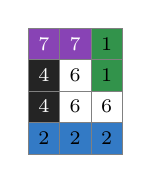
\begin{tikzpicture}[x=0.4cm,y=0.4cm]
\filldraw[fill=soma7,draw=gray,line width=.25pt] (0,0) rectangle ++(1,-1);
\node[font=\scriptsize,text=white] at (0.5,-0.5) {7};
\filldraw[fill=soma7,draw=gray,line width=.25pt] (1,0) rectangle ++(1,-1);
\node[font=\scriptsize,text=white] at (1.5,-0.5) {7};
\filldraw[fill=soma1,draw=gray,line width=.25pt] (2,0) rectangle ++(1,-1);
\node[font=\scriptsize,text=black] at (2.5,-0.5) {1};
\filldraw[fill=soma4,draw=gray,line width=.25pt] (0,-1) rectangle ++(1,-1);
\node[font=\scriptsize,text=white] at (0.5,-1.5) {4};
\filldraw[fill=soma6,draw=gray,line width=.25pt] (1,-1) rectangle ++(1,-1);
\node[font=\scriptsize,text=black] at (1.5,-1.5) {6};
\filldraw[fill=soma1,draw=gray,line width=.25pt] (2,-1) rectangle ++(1,-1);
\node[font=\scriptsize,text=black] at (2.5,-1.5) {1};
\filldraw[fill=soma4,draw=gray,line width=.25pt] (0,-2) rectangle ++(1,-1);
\node[font=\scriptsize,text=white] at (0.5,-2.5) {4};
\filldraw[fill=soma6,draw=gray,line width=.25pt] (1,-2) rectangle ++(1,-1);
\node[font=\scriptsize,text=black] at (1.5,-2.5) {6};
\filldraw[fill=soma6,draw=gray,line width=.25pt] (2,-2) rectangle ++(1,-1);
\node[font=\scriptsize,text=black] at (2.5,-2.5) {6};
\filldraw[fill=soma2,draw=gray,line width=.25pt] (0,-3) rectangle ++(1,-1);
\node[font=\scriptsize,text=black] at (0.5,-3.5) {2};
\filldraw[fill=soma2,draw=gray,line width=.25pt] (1,-3) rectangle ++(1,-1);
\node[font=\scriptsize,text=black] at (1.5,-3.5) {2};
\filldraw[fill=soma2,draw=gray,line width=.25pt] (2,-3) rectangle ++(1,-1);
\node[font=\scriptsize,text=black] at (2.5,-3.5) {2};
\end{tikzpicture}\end{minipage}\hfill
\begin{minipage}[t]{.31\linewidth}\centering{\scriptsize Felülről}\par\smallskip
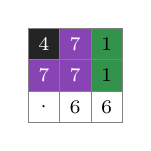
\begin{tikzpicture}[x=0.4cm,y=0.4cm]
\filldraw[fill=soma4,draw=gray,line width=.25pt] (0,0) rectangle ++(1,-1);
\node[font=\scriptsize,text=white] at (0.5,-0.5) {4};
\filldraw[fill=soma7,draw=gray,line width=.25pt] (1,0) rectangle ++(1,-1);
\node[font=\scriptsize,text=white] at (1.5,-0.5) {7};
\filldraw[fill=soma1,draw=gray,line width=.25pt] (2,0) rectangle ++(1,-1);
\node[font=\scriptsize,text=black] at (2.5,-0.5) {1};
\filldraw[fill=soma7,draw=gray,line width=.25pt] (0,-1) rectangle ++(1,-1);
\node[font=\scriptsize,text=white] at (0.5,-1.5) {7};
\filldraw[fill=soma7,draw=gray,line width=.25pt] (1,-1) rectangle ++(1,-1);
\node[font=\scriptsize,text=white] at (1.5,-1.5) {7};
\filldraw[fill=soma1,draw=gray,line width=.25pt] (2,-1) rectangle ++(1,-1);
\node[font=\scriptsize,text=black] at (2.5,-1.5) {1};
\filldraw[fill=white,draw=gray,line width=.25pt] (0,-2) rectangle ++(1,-1);
\node[font=\scriptsize] at (0.5,-2.5) {$\cdot$};
\filldraw[fill=soma6,draw=gray,line width=.25pt] (1,-2) rectangle ++(1,-1);
\node[font=\scriptsize,text=black] at (1.5,-2.5) {6};
\filldraw[fill=soma6,draw=gray,line width=.25pt] (2,-2) rectangle ++(1,-1);
\node[font=\scriptsize,text=black] at (2.5,-2.5) {6};
\end{tikzpicture}\end{minipage}
\end{center}
\end{minipage}\par\medskip

\end{multicols}
\end{document}
